\section{Muestras obtenidas}

La implementación del sistema da como resultado un total de 178 videos tomados, de los cuales solo fueron procesados un total de 29 videos, la baja cantidad de videos procesados fue debido al tiempo de ejecución del sistema, además de que en algunos casos había que volver a procesar un mismo video varias veces, el sistema procesa entre 30 y 45 fotogramas por segundo lo cual se traduce en el mejor de los casos en 1.333 segundos procesar un segundo real de video.

Los 29 videos procesados dieron un total de 532 muestras, con datos se realizaron los experimentos. Para los experimentos los datos fueron separados por carril 0, 1 y 2, los cuales representan el primer carril, carril central y último carril. Los datos para cada carril son los siguientes:

\begin{itemize}
    \item Primer carril: 8 datos (Figura \ref{fig:carril_0})
    \item Carril central: 239 datos (Figura \ref{fig:carril_1})
    \item Último carril: 285 datos (Figura \ref{fig:carril_2})
\end{itemize}

\begin{figure}[H]
    \centering
    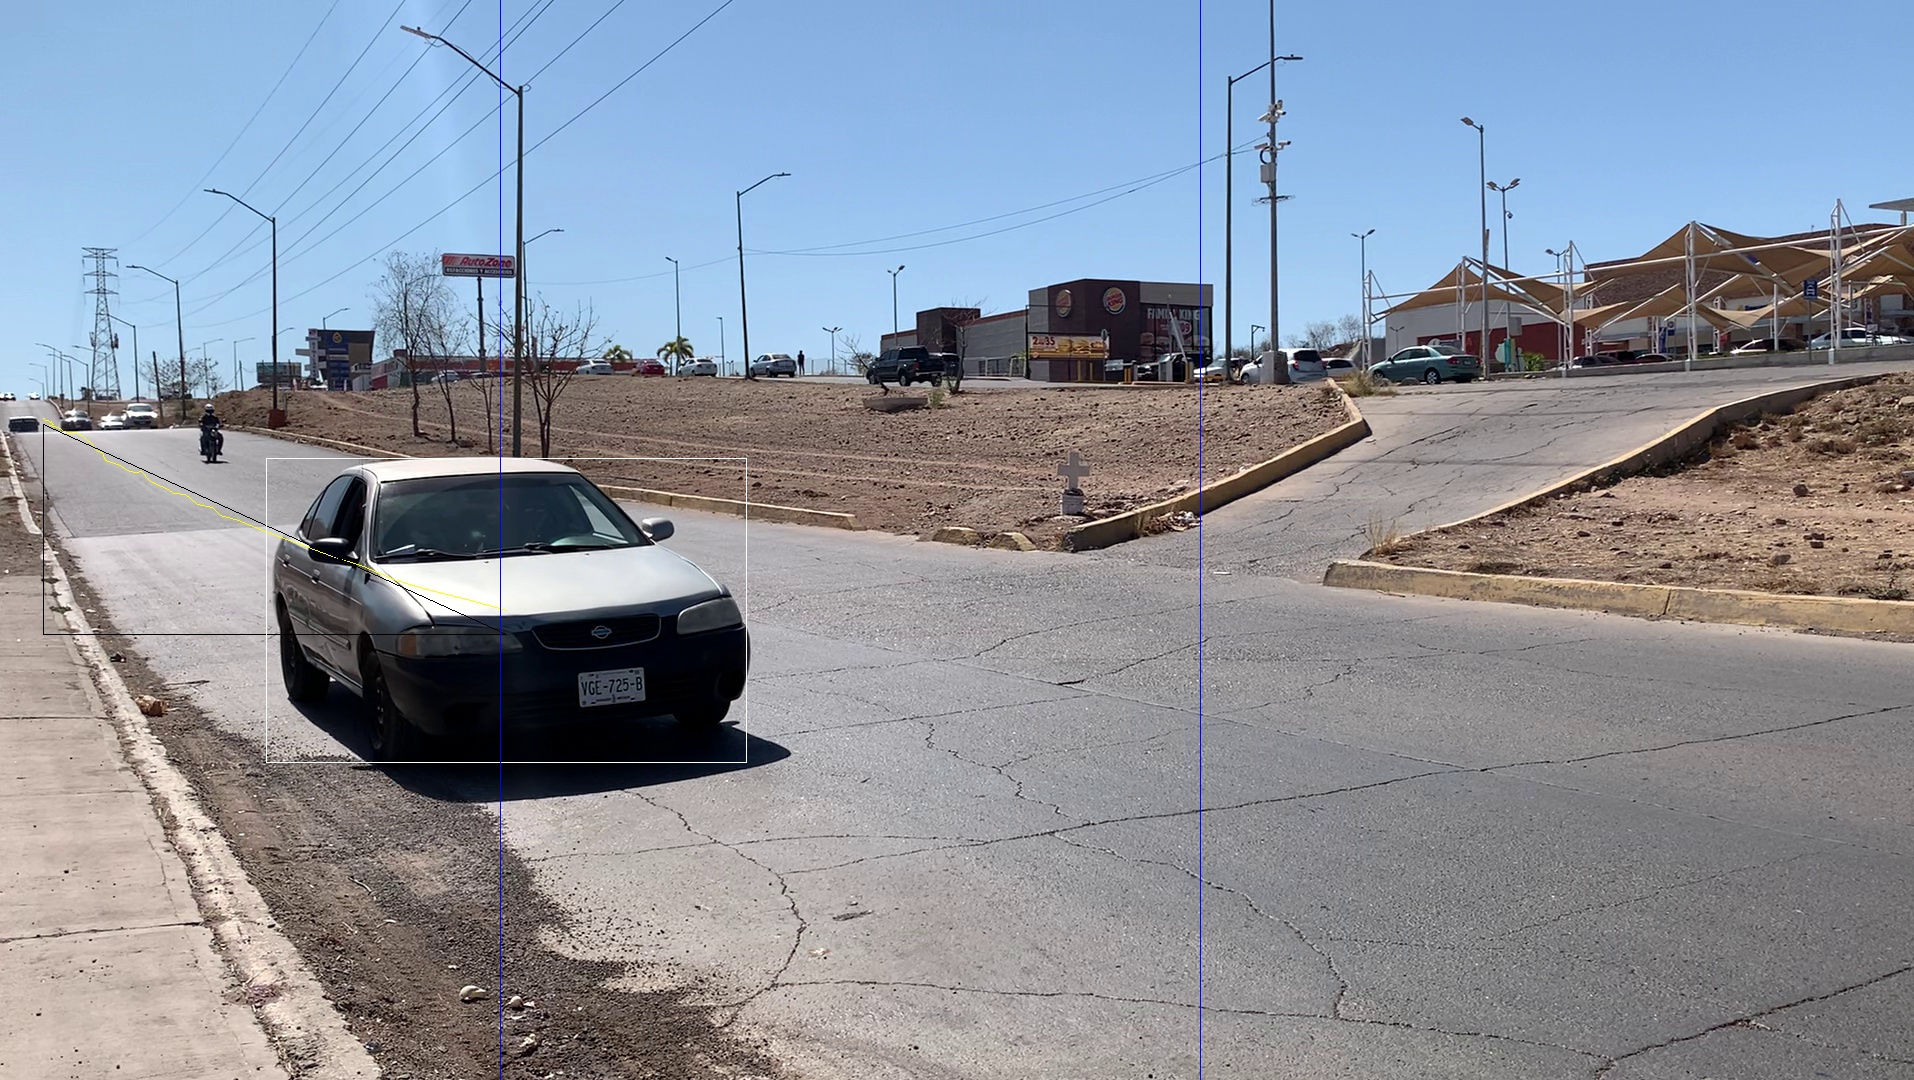
\includegraphics[width=0.8\textwidth]{Resultados/imgs/carril_0.jpg}
    \caption{Muestra de primer carril.}
    \label{fig:carril_0}
\end{figure}

\begin{figure}[H]
    \centering
    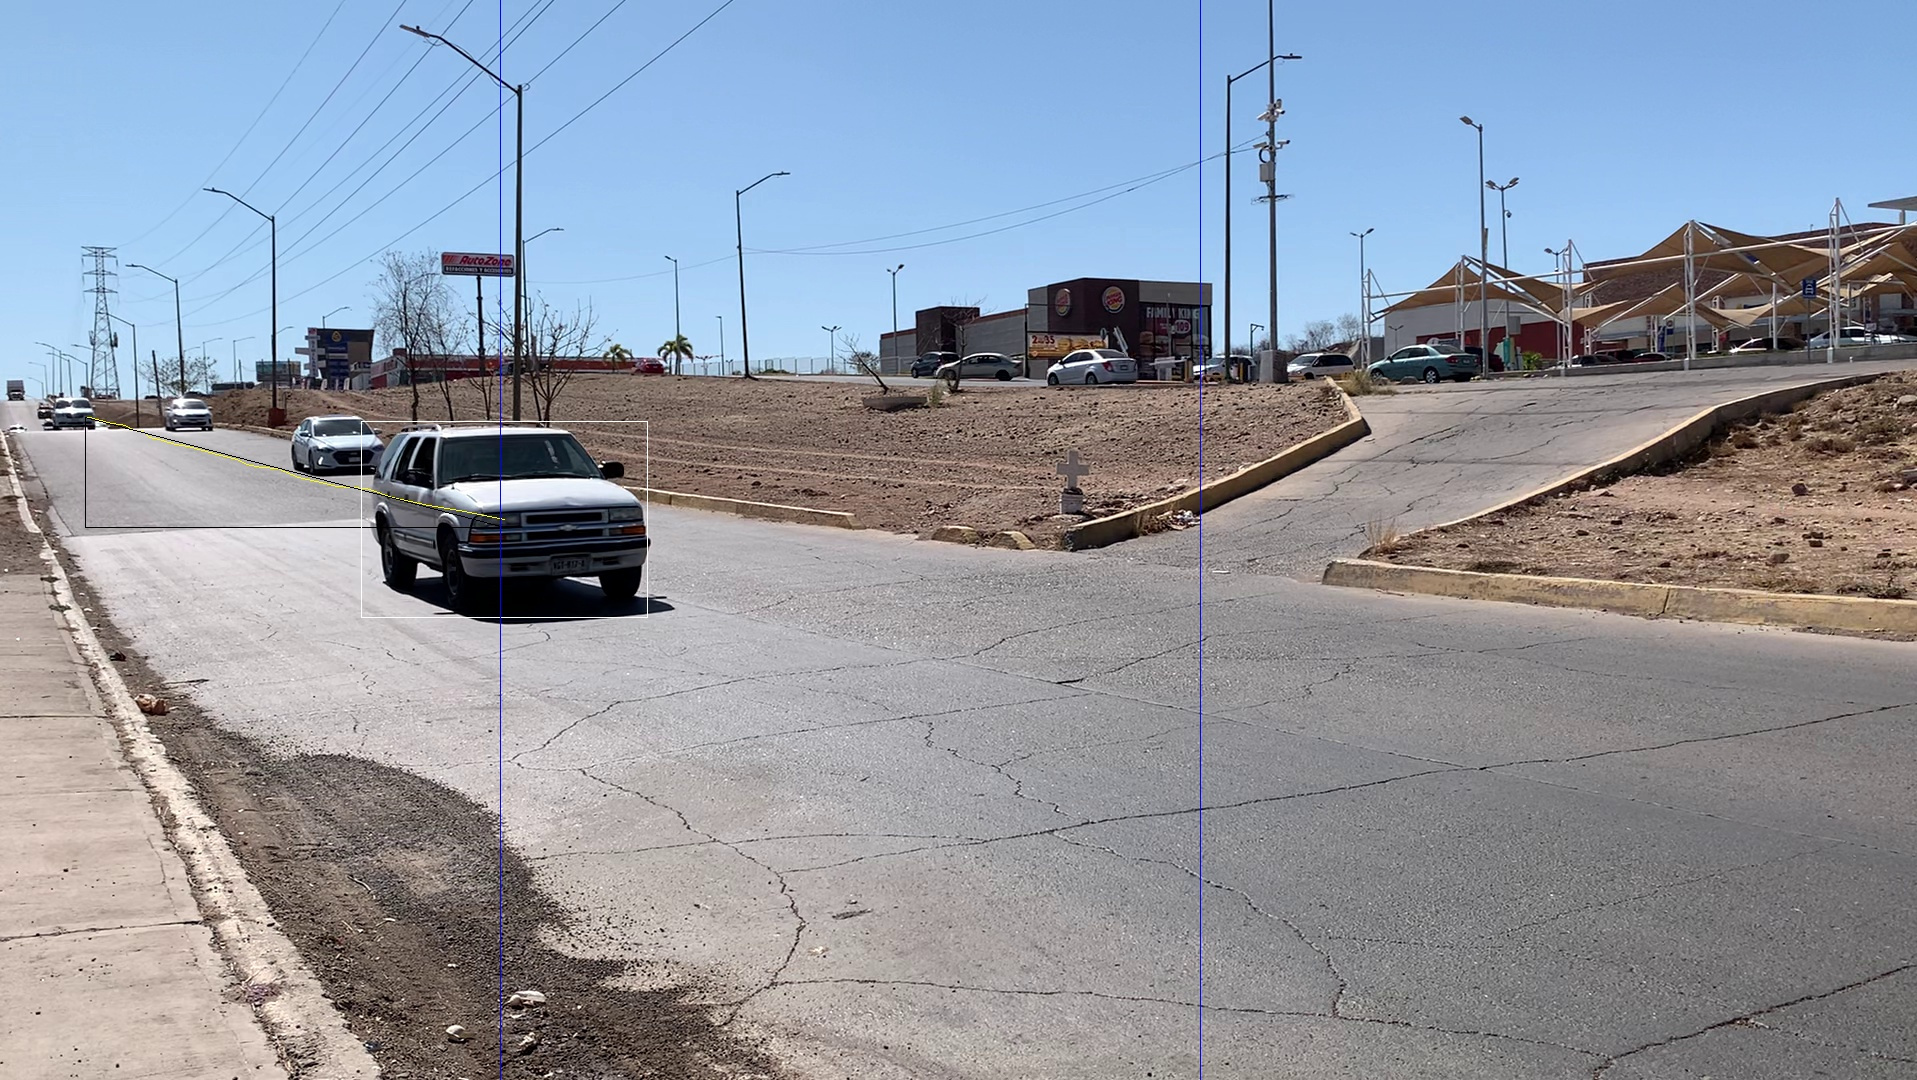
\includegraphics[width=0.8\textwidth]{Resultados/imgs/carril_1.jpg}
    \caption{Muestra de segundo carril.}
    \label{fig:carril_1}
\end{figure}

\begin{figure}[H]
    \centering
    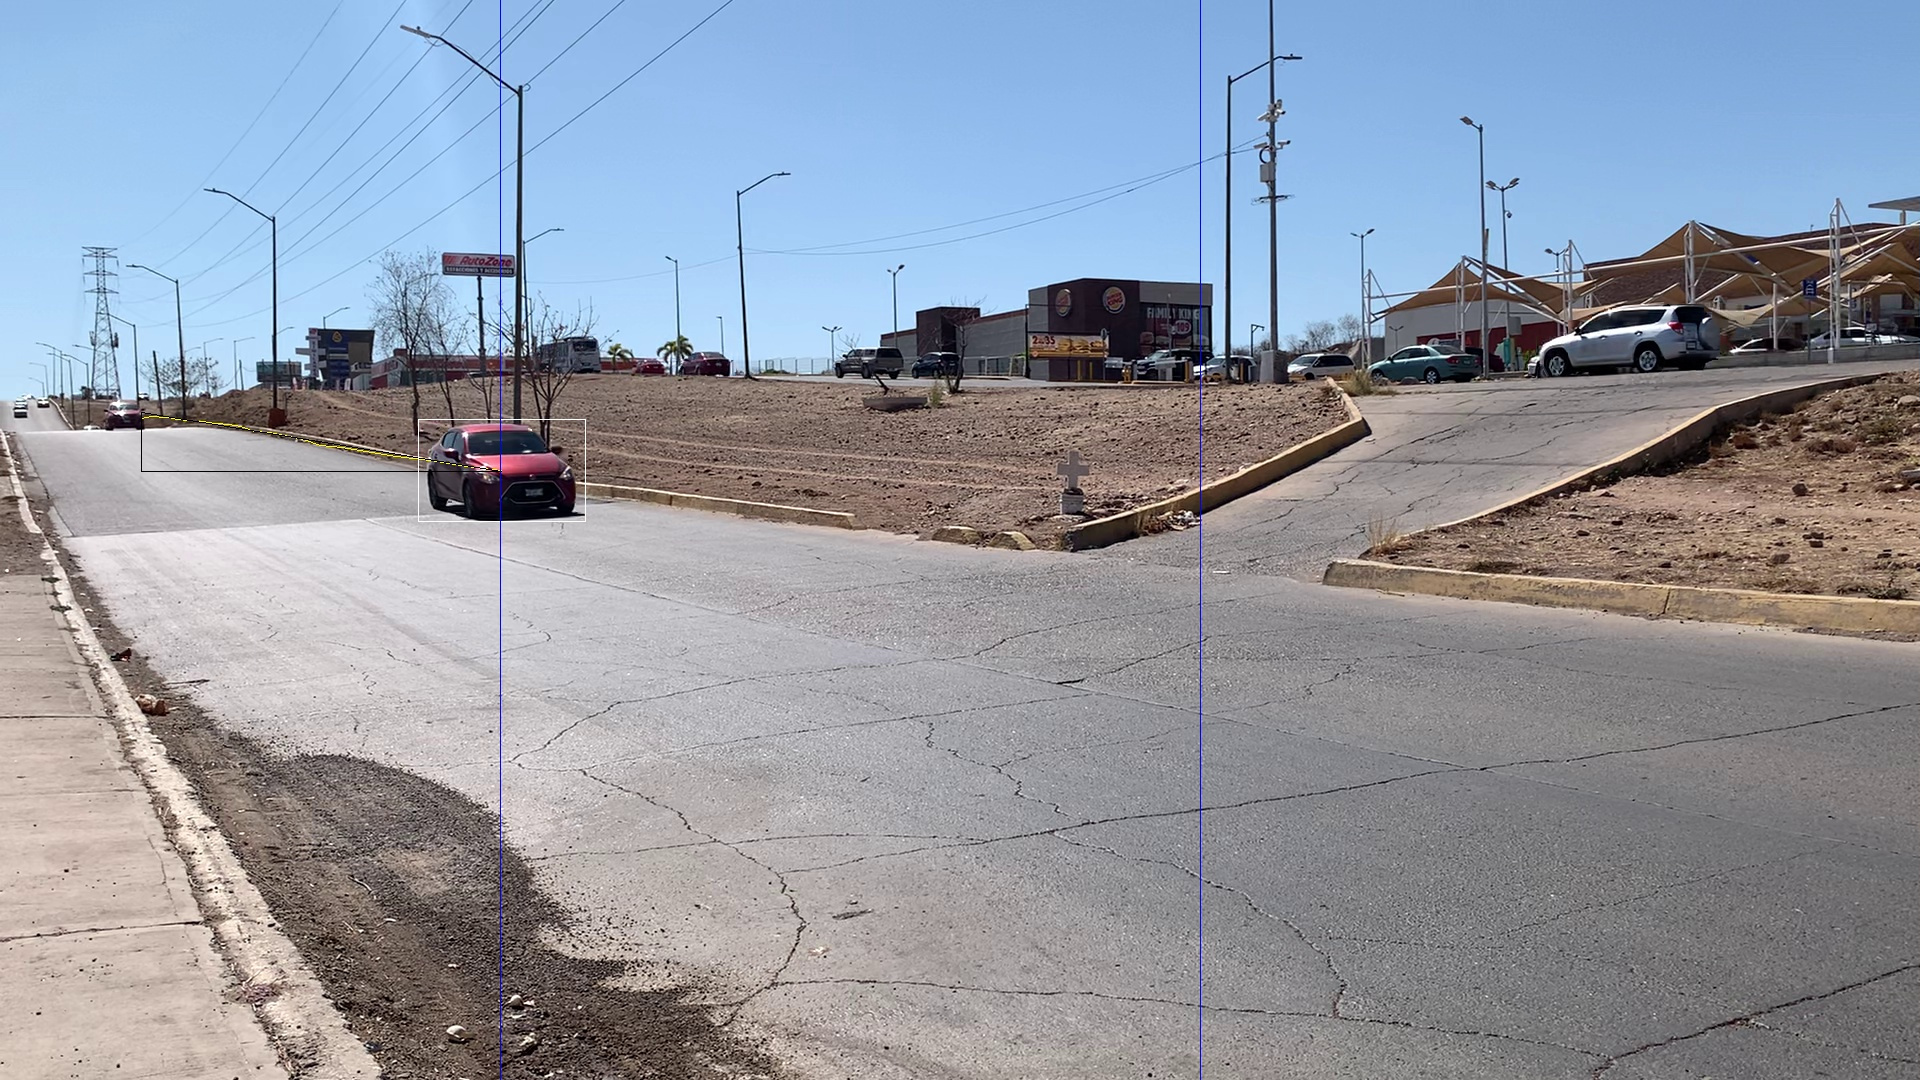
\includegraphics[width=0.8\textwidth]{Resultados/imgs/carril_2.jpg}
    \caption{Muestra de último carril.}
    \label{fig:carril_2}
\end{figure}

Como se nota la diferencia del número de datos para el primer carril es considerablemente bajo con respecto a los otros dos carriles, por lo cual se omiten los experimentos para este carril, dejando solamente el cerril central y el último carril.
